\documentclass{beamer}
%[aspectratio=169] \usepackage[czech]{babel}
\usepackage{apo-lecture-en}
\usepackage{pdfpages}
\usepackage{pdfcomment}
\usepackage{listings}
\usepackage{array,multirow}

\subtitle{Lecture 06. Branch and Speculative Execution}
\author{Pavel Píša \phantom{xxxxxxx} Petr Štěpán \\ \small\texttt{pisa@fel.cvut.cz} \phantom{xx} \small\texttt{stepan@fel.cvut.cz} \\
\phantom{xxxxxxxxx} \\
License: CC-BY-SA}
\begin{document}

\maketitle

\section{Superscalar architecture}

\begin{frame}
\frametitle{Today's lecture objective}

\begin{itemize}
 \item A look at another possible processor speedup that builds on pipelining -- the superscalar architecture
 \item Jump prediction as a very important feature of superscalar processors
 \item Both of these techniques are used in RISC-V processors as well as in all current processors
\end{itemize}

\end{frame}

\begin{frame}[fragile]
\frametitle{Recap - quiz}

In which case do the instructions cause a data hazard?

\begin{columns}[T]
\begin{column}{0.40\textwidth}
\phantom{xxxxx}a)

\begin{minted}[fontsize=\footnotesize]{gas}
addi t0, s1, 4
add  t1, s1, s0
add  s1, s2, x0
\end{minted}
\end{column}
\begin{column}{0.40\textwidth}
\phantom{xxxxx}b)

\begin{minted}[fontsize=\footnotesize]{gas}
addi t0, s1, 4
add  t1, s2, s3
add  t2, t0, t1
\end{minted}
\end{column}
\end{columns}
\bigskip
\begin{itemize}
 \item[A] in neither column
 \item[B] hazard is only in case a)
 \item[C] hazard is only in case b)
 \item[D] hazard is in case a) and b)
\end{itemize}

\end{frame}

\begin{frame}[fragile]
\frametitle{Recap - quiz}

How can the following data hazard be solved?

\begin{minted}[fontsize=\footnotesize]{gas}
lw   s2, 10(s0)
addi s1, s2, -1
\end{minted}
\bigskip
\begin{itemize}
 \item[A] this hazard cannot be solved, it must be solved by the compiler or programmer
 \item[B] can be solved by data forwarding
 \item[C] must only be resolved using stall
 \item[D] can be solved by a combination of stall and data forwarding
\end{itemize}

\end{frame}


\begin{frame}

\frametitle{Processor with pipeline (from lecture 5)}

How can the Hazard Unit make a decision about data hazard when it's causing problems for students? Simple:
\begin{columns}
\begin{column}{0.67\textwidth}
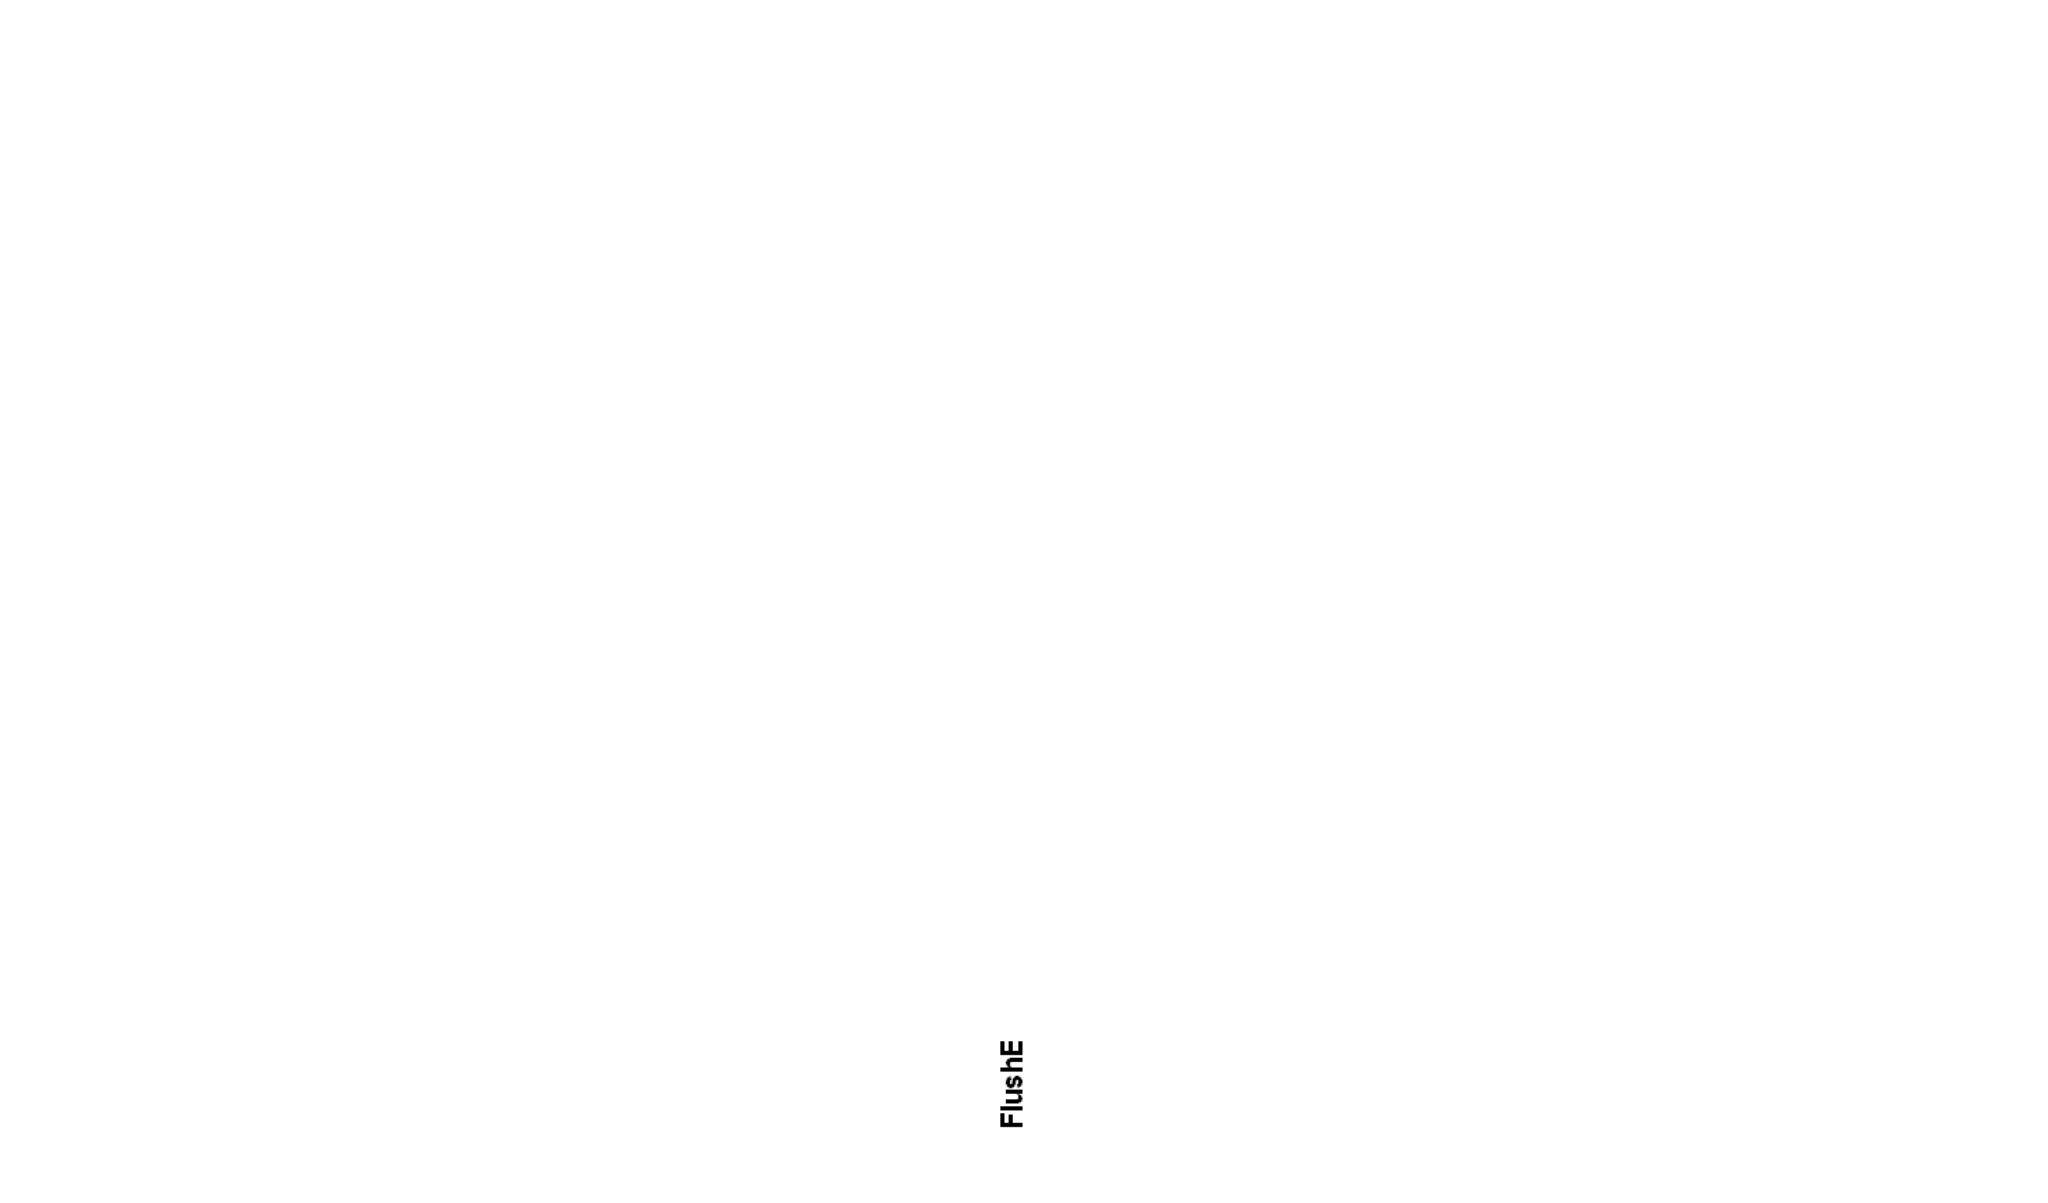
\includegraphics[width=\textwidth]{cpu_final_design.pdf}
\end{column}
\begin{column}{0.33\textwidth}
\footnotesize
\begin{itemize}
\item If RegWriteM==1, MemToRegM==0 and WriteRegM==RsE1 or RsE2 then set ForwardAE to 2 or ForwardBE to 2
\item If RegWriteW==1, MemToRegW==0 and WriteRegW==RsE1 or RsE2 then set ForwardAE to 1 or ForwardBE to 1
\end{itemize}
\end{column}
\end{columns}
\bigskip
\footnotesize
\begin{itemize}
\item If MemToRegM==1 and WriteRegW==Rs1E or Rs2E then set suspend - STALL
\end{itemize}
\end{frame}

\begin{frame}
\frametitle{Instruction-level parallelism}

Instruction Level Parallelism (ILP)
\begin{itemize}
 \item Pipelining -- different phases of different instructions are processed in parallel
 \item Superpipelining -- superpipelining refers to pipelining with more than 10 steps. Slower pipelining phases are split into multiple parts, allowing the processor to increase its frequency and thus its performance.
 \item Superscalar processor -- the same stages of different instructions are processed in parallel
\begin{itemize}
\item we can have multiple ALUs and execute in parallel EX phases of multiple different instructions
\item in the fetch phase we can fetch multiple instructions in parallel in succession, i.e. instructions from address PC, PC+4, PC+8 and PC+12
\item the individual instruction phases are additionally chained, so that after fetching 4 instructions in parallel, we fetch the next 4 instructions directly
\end{itemize}
\end{itemize}

\end{frame}

\begin{frame}
\frametitle{Instruction-level parallelism}

Pipelined processor
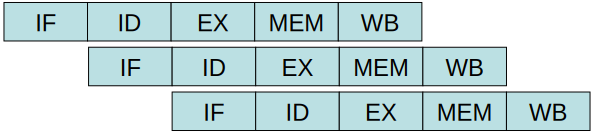
\includegraphics[width=0.85\textwidth]{pipeline.pdf}

Superscalar processor
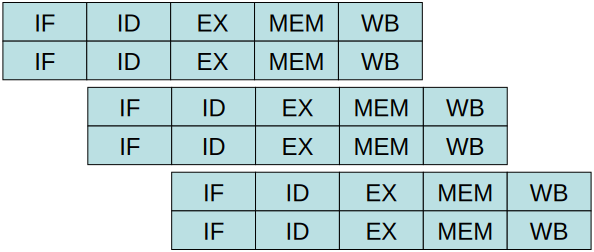
\includegraphics[width=0.85\textwidth]{superscalar.pdf}

\end{frame}

\begin{frame}
\frametitle{Superscalar processors}

\begin{itemize}
\item Superscalar processors have an IPC (Instruction Per Clock) greater than 1.
  \begin{itemize}
  \item Normal and pipelined processors have IPC=1 all the time
  \end{itemize}
\item The number of parallel branches is called the instruction pipeline width.
\item There are two basic variants:
  \begin{itemize}
  \item \textbf{Static} superscalar architecture -- only consecutive instructions in a program can run in parallel.
    \begin{itemize}
    \item If instructions depend on each other, this leads to a processor stall.
    \end{itemize}
  \item \textbf{Dynamic} superscalar architecture -- any instructions that are ready to execute can run in parallel.
    \begin{itemize}
    \item Allows instructions to be preempted by out-of-order execution.
    \item Makes better use of the processor's HW resources.
    \end{itemize}
  \end{itemize}
\end{itemize}

\end{frame}

\begin{frame}
\frametitle{Superscalar processors}

\begin{itemize}
\item Individual parallel branches can be \textbf{unified} -- that is, all branches are the same and can perform all types of operations
  \begin{itemize}
  \item In practice, this would be an unnecessarily complex processor -- it is not used
  \end{itemize}
\item The individual parallel branches are \textbf{specialized} -- each branch can only do certain instructions:
  \begin{itemize}
  \item register-only instructions -- calculations, comparisons
  \item instructions working with memory -- loading/loading data from/to memory
  \item jump instructions -- PC changing instructions
  \end{itemize}
\end{itemize}
\end{frame}

\section{Register Computation Reorganization}

\begin{frame}
\frametitle{Superscalar Architecture}
\begin{columns}
\begin{column}{0.55\textwidth}
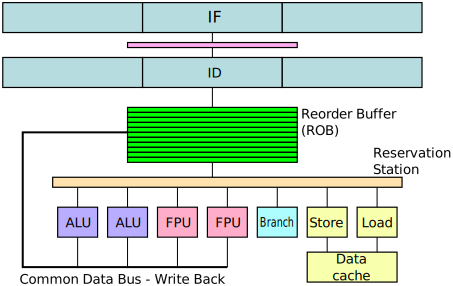
\includegraphics[width=\textwidth]{superscalar-architecture.pdf}
\end{column}
\begin{column}{0.45\textwidth}
\begin{itemize}
\item The basis of the architecture is the ReOrder Buffer (ROB), which can improve instruction parallelization by renaming registers.
\item Reservation Station extends the possibilities of storing operands for operations and organizes their execution
\item Common Data Bus ensures that calculated values are written to the actual registers even for renamed registers.
\end{itemize}
\end{column}
\end{columns}
\end{frame}


\begin{frame}[fragile]
\frametitle{Data hazards in superscalar architecture}

For register-only instructions:
\begin{itemize}
\item is clear that it is not possible to execute all instructions in parallel
\item is possible to increase parallelization by using a hidden set of registers.
\end{itemize}

\begin{minted}[fontsize=\footnotesize]{gas}
1: slli t1, s1, 4
2: add  t0, t1, s2
3: addi s2, t0, 8
4: mult t1, s0, s0
5: addi t3, t1, 100
\end{minted}

This program can be parallelized using a hidden set of registers for renaming:

\begin{columns}[T]
\begin{column}{0.40\textwidth}
\begin{minted}[fontsize=\footnotesize]{gas}
1: slli RN0, s1,  4
2: add  RN1, RN0, s2
3: addi RN2, RN1, 8
\end{minted}
\end{column}
\begin{column}{0.40\textwidth}
\begin{minted}[fontsize=\footnotesize]{gas}
4: mult RN3, s0,  s0
5: addi RN4, RN3, 100
\end{minted}
\end{column}
\end{columns}
\end{frame}


\begin{frame}
\frametitle{Tomasulo algorithm}

Robert Tomasulo from IBM invented an algorithm for out-of-order computation on FPUs in 1967.
Today, a modification of it is the basis of the architecture of all modern processors.
The basic stages are:
\begin{itemize}
\item Introducing an instruction into the ROB and renaming the result register of the operation - getting the register number from the backup register file.
\item Load the instruction into the Reservation Station and wait for the prepared data
\item Performing the calculation and writing the result to the renamed register via the Common Data Bus
\item Completing the oldest instruction (circular queue -- FIFO) from the ROB and updating the system register.
\end{itemize}
Instructions may be computed out-of-order, but instruction completion is in program order.
\end{frame}

\begin{frame}
\frametitle{Superscalar Architecture}

\begin{center}
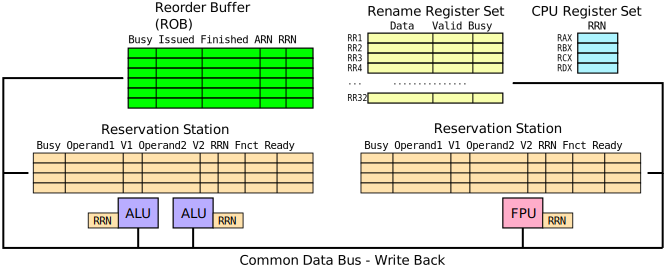
\includegraphics[width=0.7\textwidth]{superscalar-architecture2.pdf}
\end{center}

\scriptsize
Rename Register Set:
\begin{itemize}
\item A set of auxiliary registers, often many times the number of CPU registers.
\item The Busy flag indicates that the register is being used, the Valid flag indicates that the value is calculated and is valid. When the instruction completes, the CPU register is set to RRN.
\end{itemize}

ReOrder Buffer:
\begin{itemize}
\item The cyclic queue contains instructions inserted in program order
\item The queue ensures that instructions are completed in program order
\item Binding between Reservation Station via Rename Register Number (RRN Rename Register Number), which will contain the result of the operation
\item Via the Common Data Bus it learns that the RRN register has been calculated and the instruction gets the Finished flag
\item Finish instruction - removes only the oldest instruction from the ROB when it gets the finish flag.
\end{itemize}


\end{frame}

\begin{frame}
\frametitle{Superscalar architecture}

\begin{center}
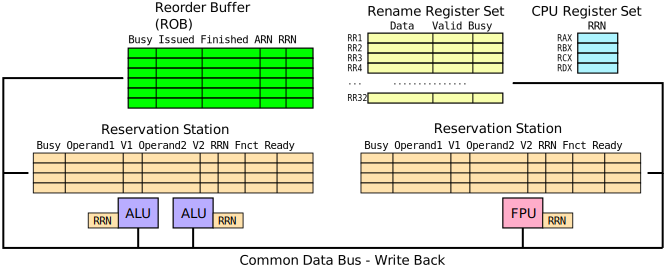
\includegraphics[width=0.7\textwidth]{superscalar-architecture2.pdf}
\end{center}

\scriptsize
Reservation Station:
\begin{itemize}
\item Contains two operands, if the V1/2 flag is set then the operand value is valid. If the V1/2 flag is not set, then the operand contains an RRN whose value is being waited for and received from the CDB
\item The RRN number indicates which register to write the result to.
\item If both operands are valid and the ALU/FPU is free, the operation is entered and the item is removed from the Reservation Station (the RRN of the result is remembered so that the ALU/FPU can send it to the Common Data Bus)
\end{itemize}

\end{frame}

\begin{frame}
\frametitle{Memory read data hazards}

\begin{itemize}
\item If the lw and sw instructions use different addresses, we can swap them.
\item If lw follows sw from the same address, data forwarding can be implemented.
\item In practice, however, one instruction may overtake the other, so that it is not yet calculated where the data will be stored, i.e. whether a hash will occur.
\begin{itemize}
\item Solution - speculative execution of the lw instruction, i.e. execution even though it is not clear whether the data will be correct
\item When the sw instruction completes, all speculative executions of lw are checked
\item When a conflict is found, speculative execution of the lw instruction is cancelled
\end{itemize}
\item Execution is treated as if the order is preserved.
\item A big problem in multiprocessor systems -- memory consistency when parallel computations are performed on different processor cores.
\end{itemize}

\end{frame}



\begin{frame}
\frametitle{AMD Zen2 - Microarchitecture}

\begin{columns}[T]
\begin{column}{0.34\textwidth}
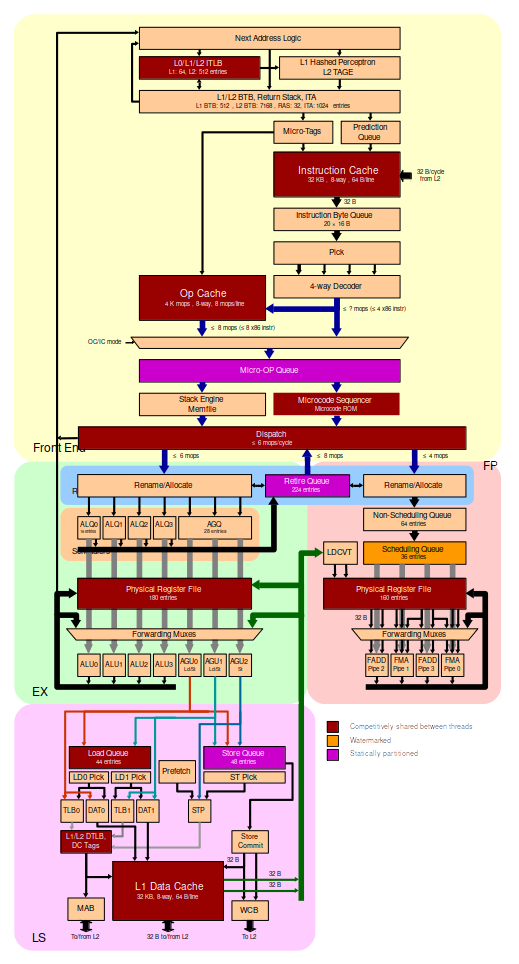
\includegraphics[width=\textwidth]{fig/amd_zen2.png}
\end{column}
\begin{column}{0.66\textwidth}
\scriptsize
\begin{itemize}
\item 7 nm process (from 12 nm), I/O die utilizes 12 nm
\item Core (8 cores on CPU chiplet), 6/8/4 µOPs in parallel
\begin{itemize}
\scriptsize
\item Frontend, µOP cache (4096 entries)
\item FPU, 256-bit Eus (256-bit FMAs) and LSU (2x256-bit L/S), 3 cycles DP vector mult latency
\item Integer, 180 registers, 3x AGU, scheduler (4x16 ALU + 1x28 AGU)
\item Reorder Buffer 224 entries
\end{itemize}
\item Memory subsystem
\begin{itemize}
\scriptsize
\item L1 i-cache and d-cache, 32 KiB each, 8-way associative
\item L2 512 KiB per core, 8-way,
\item L2 DTLB 2048-entry
\item 48 entry store queue
\end{itemize}
\end{itemize}
Autor: QuietRub\\
Source: \url{https://en.wikichip.org/wiki/amd/microarchitectures/zen_2}
\end{column}
\end{columns}

\end{frame}


\begin{frame}
\frametitle{Recap - quiz}

What is a control hazard?

\bigskip
\begin{itemize}
 \item[A] hazard that must be addressed by data forwarding
 \item[B] hazard that must be handled by stall
 \item[C] a situation in which the currently processed instruction must be discarded
 \item[D] the problem of unstable results of logical operations
\end{itemize}
\end{frame}

\section{Jump predictors}


\begin{frame}
\frametitle{Control hazards in Superscalar Architecture}

\begin{itemize}
\item Jumps in the program change which instructions are executed.
\item With conditional jumps, it is not clear which instructions will be executed.
\item Calculating the condition for a jump can take a long time, there are many instructions in progress.
\begin{itemize}
\item Solution - speculative loading of additional instructions
\item After all the calculations necessary for the jump decision have been completed, it is checked whether or not to jump.
\item If the prediction is wrong, many instructions in progress or even speculatively executed must be discarded.
\end{itemize}
\item Even unconditional jumps have trouble calculating where to jump. The destination of a jump may depend on the computation of previous instructions, and therefore cannot be easily determined when fetching instructions.
\begin{itemize}
\item Solution - speculatively guess what address to jump to, based on the history of past jumps.
\item After all calculations are done, check if the correct address has been guessed.
\item Especially important for returning from a function.
\end{itemize}
\end{itemize}

\end{frame}


\begin{frame}
\frametitle{Superscalar Architecture Control hazards}

\begin{itemize}
\item A jump is statistically every 4 to 7 instructions in the program
\item 20\% of jumps are unconditional -- they always jump, no need to decide
\item 80\% of jumps are conditional
  \begin{itemize}
  \item about 66\% are jumps to a higher address, or forward
    \begin{itemize}
    \item these jumps correspond to branching type \texttt{if}
    \item of these, statistically about 60\% are not jumped -- we will denote \textbf{NT} (Not Taken)
    \end{itemize}
  \item the rest about 34\% are jumps to a lower address, or backwards
    \begin{itemize}
    \item these jump correspond to jumps of the type \texttt{for}, \texttt{while} and \texttt{do ... while}
    \item of these, statistically 99\% (almost all) will jump -- we will denote \textbf{T} (Taken)
    \end{itemize}
  \end{itemize}
\end{itemize}

\end{frame}


\begin{frame}
\frametitle{Static predictors}

Static predictors always have the same result for a given jump instruction:
\begin{itemize}
\item A predictor that would always estimate that it always jumps
\begin{itemize}
\item According to the statistics on the previous page, it would have a success rate of $p_{taken} = (0.66*0.4+0.34*0.99) = 0.60$
\item Statistically, it turns out that $p_{taken}$ is in the range of 60 -- 70\% for most programs.
\end{itemize}
\item BTFNT predictor -- Backwards Taken / Forwards Not Taken
\begin{itemize}
\item According to the sign of the relative jump - backward jump is jumped, forward jump is not jumped
\item According to the stats on the previous page, it would have a success rate of $p_{taken} = (0.66*0.6+0.34*0.99) = 0.73$
\end{itemize}
\end{itemize}

\end{frame}

\begin{frame}[fragile]
\frametitle{Static predictor BTFNT}

Example of translating a \texttt{for} cycle:

\begin{columns}[T]
\begin{column}{0.4\textwidth}
\begin{minted}{c}
for (i=0; i<N; i++) {

  ...
  
}
\end{minted}
\end{column}
\begin{column}{0.6\textwidth}
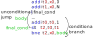
\includegraphics[width=\textwidth]{for_cykle-en.pdf}
\end{column}
\end{columns}
\bigskip
For a conditional jump, $N-1$ times jumps and $1$ does not jump.\\
It jumps backwards and the probability of a correct prediction is $\frac{N-1}{N}$

\end{frame}

\begin{frame}[fragile]
\frametitle{Static predictor BTFNT}

Example of translating the \texttt{if else} construct:

\begin{columns}[T]
\begin{column}{0.4\textwidth}
\begin{minted}{c}
if (a<b) {
  
  ...

} else {

  ...

}
\end{minted}
\end{column}
\begin{column}{0.6\textwidth}
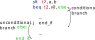
\includegraphics[width=\textwidth]{if_translation-en.pdf}
\end{column}
\end{columns}
\bigskip
The unconditional jump depends on the values of a, b, so nothing can be said about it in general, except that it always jumps forward.\\
The statistical behavior depends on the type of program, but for a mixture of different programs it turns out that the probability of a jump is $0.4$.

\end{frame}


\begin{frame}
\frametitle{Dynamic predictors}

\small
Dynamic predictors try to estimate whether a jump will occur based on the past behavior of a given jump instruction:
\begin{itemize}
\item It would be ideal if each jump instruction had its own predictor
\begin{itemize}
\small
\item But this is not possible, a jump instruction can be at any location in 4GiB memory
\end{itemize}
\end{itemize}


\begin{columns}[T]
\begin{column}{0.5\textwidth}
\small
Solution: we will have $2^k$ predictors and select a predictor according to the $k$ lowest bits of the jump instruction address
\begin{itemize}
\item Some jump instructions at different addresses but with the same lowest $k$ bits of the address will interfere -- \textbf{interfere}.
\item Interference can very adversely affect prediction success.
\end{itemize}
\end{column}
\begin{column}{0.5\textwidth}
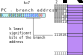
\includegraphics[width=\textwidth]{prediction_table-en.pdf}
\end{column}
\end{columns}

\end{frame}


\begin{frame}
\frametitle{1-bit Smith predictor}

The simplest predictor is the 1-bit Smith predictor
\begin{itemize}
\item Has only two states, switches according to past behavior
\item Predicts that it will turn out the way it did last time.
\begin{itemize}
\item very simple to implement, evaluate and adjust to reality
\end{itemize}
\end{itemize}

\begin{center}
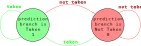
\includegraphics[width=0.45\textwidth]{smith_1bit-en.pdf}
\end{center}

\end{frame}

\begin{frame}[fragile]
\frametitle{1-bit Smith predictor}

Prediction of the for loop:

\begin{columns}[T]
\begin{column}{0.35\textwidth}
\begin{minted}{c}
for (i=0; i<5; i++) {
  ...
}
\end{minted}
\end{column}
\hfill
\begin{column}{0.45\textwidth}
\begin{minted}{gas}
      addi t0, x0, 0
      addi t1, x0, 5
      j cond
body: ...
      addi t0, t0, 1
cond: slt  t2, t0, t1
      bne  t2, x0, body
\end{minted}
\end{column}
\end{columns}
\bigskip
If the predictor does not interfere with other jumps, then it starts in state 0 -- NT (Not taken).

\begin{tabular}{|l|c|c|c|c|c|c|}\hline
Real behaviour & T & T & T & T & T & NT\\\hline
Prediction & {\color{red}NT} & T & T & T & T & {\color{red}T}\\\hline
\end{tabular}

You can see that the predictor is not successful at the beginning of the for loop and at the end.

The success rate of the 1-bit Smith predictor for a loop with $r$ iterations is $\frac{r-2}{r}$.
\end{frame}


\begin{frame}
\frametitle{2-bit Smith predictor}

The 2-bit Smith predictor is still one of the simplest
\begin{itemize}
\item It already has 4 states, represented by 2 bits.
\item 2 states predict a jump, 2 states predict a non-jump
\item Prediction depends on past behaviour, but tolerates one deviation from regularity
\item Very simple to implement, evaluate and adjust to reality
\end{itemize}

\begin{center}
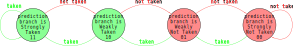
\includegraphics[width=0.95\textwidth]{smith_2bit-en.pdf}
\end{center}
\end{frame}

\begin{frame}[fragile]
\frametitle{2-bit Smith predictor}

Prediction for for loop:

\begin{columns}[T]
\begin{column}{0.35\textwidth}
\begin{minted}{c}
for (i=0; i<5; i++) {
  ...
}
\end{minted}
\end{column}
\hfill
\begin{column}{0.45\textwidth}
\begin{minted}{gas}
      addi t0, x0, 0
      addi t1, x0, 5
      j cond
body: ...
      addi t0, t0, 1
cond: slt  t2, t0, t1
      bne  t2, x0, body
\end{minted}
\end{column}
\end{columns}
\bigskip
\small
If the predictor does not interfere with other jumps, then it starts in state 10 -- WT (Weakly taken).

\begin{tabular}{|l|c|c|c|c|c|c|c|}\hline
Real behaviour & T & T & T & T & T & NT & \\ \hline
State & WT & ST & ST & ST & ST & ST & WT\\ \hline
Prediction & T & T & T & T & T & {\color{red}T} &\\\hline
\end{tabular}

You can see that the predictor is not successful only at the end of the for loop.

The success rate of the 2-bit Smith predictor for a loop with $r$ iterations is $\frac{r-1}{r}$.
\end{frame}


\begin{frame}
\frametitle{2-bit Smith predictor with hysteresis}

Analogue of the 2-bit Smith predictor
\begin{itemize}
\item When two changes occur in succession, it goes straight to the Strongly state and two more opposite behaviors must occur in succession for the predictor to flip to the new state.
\end{itemize}

\begin{center}
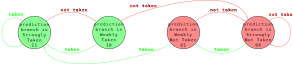
\includegraphics[width=0.95\textwidth]{smith_2bit_hist-en.pdf}
\end{center}
\end{frame}


\begin{frame}
\frametitle{Predictor evaluation}

\begin{itemize}
\item It's impossible to decide in general when a predictor is better. It is always possible to find counterexamples where each of the predictors behaves best
\item The only possibility is a statistical analysis of different programs:
\end{itemize}
\begin{center}
\begin{tabular}{|l|c|} \hline
Static predictor - always jumps & 59.25 \\\hline
1-bit Smith predictor & 68.75 \\\hline
2-bit Smith predictor with hysteresis & 81.75 \\\hline
\end{tabular}
\end{center}

Source: \url{https://ieeexplore.ieee.org/document/6918861}\\
H. Arora, S. Kotecha and R. Samyal, "Dynamic Branch Prediction Modeller for RISC Architecture," 2013 International Conference on Machine Intelligence and Research Advancement, Katra, 2013, pp. 397-401.
\end{frame}

\begin{frame}[fragile]
\frametitle{Prediction dependence}

In practice, it turns out that the prediction depends on the previous behavior of the program.

\begin{minted}{c}
if (x==2) { // jump s1
}
if (y==2) { // jump s2
}
if (x!=y) { // jump s3
}
\end{minted}

If the variables \texttt{x}, \texttt{y} do not change in the bodies of the conditions \texttt{s1} and \texttt{s2}, then we have a strong dependency of the jump \texttt{s3}:

\bigskip

\begin{tabular}{|l|l|l|l|l|l|}\hline
s1 & s2 & $\implies$ s3 & explanation \\\hline
doesn't jump & jumps & doesn't jump & x==2 & y!=2 therefore x!=y \\\hline
jumps & doesn't jump & doesn't jump & x!=2 & y==2 therefore x!=y \\\hline
does not jump & does not jump & jumps & x==2 and y==2 therefore x!=y\\\hline does not apply
jumps & jumps & we don't know & x!=2 and y!=2 we don't know if x!=y \\\hline
\end{tabular}
\end{frame}



\begin{frame}
\frametitle{Jump history -- correlated predictors}

The Branch Histrory Register (BHR) contains information about whether the last $m$ jumps made a jump:
\begin{itemize}
\item If jumped then contains 1, if not jumped then contains 0
\item The new information is inserted at the lowest bit, the oldest information is discarded from the highest position, the other information is shifted.
\end{itemize}

\begin{columns}[T]
\begin{column}{0.5\textwidth}
\small
To find the predictor index, the $k-m$ lowest bits of the jump instruction address are taken and this information is concatenated with the bits from the BHR
\begin{itemize}
\item Advantage -- a different predictor is selected based on the previous jumps.
\item Disadvantage -- some combinations do not occur in the BHR and therefore these predictors are not used.
\end{itemize}
\end{column}
\begin{column}{0.5\textwidth}
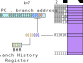
\includegraphics[width=\textwidth]{prediction_BHR-en.pdf}
\end{column}
\end{columns}

\end{frame}

\begin{frame}
\frametitle{GShare predictors}

The GShare approach is similar to the previous one:
\begin{itemize}
\item It also uses the BHR register, which in this implementation has directly $k$ bits
\end{itemize}

\begin{columns}[T]
\begin{column}{0.5\textwidth}
\small
To find the predictor index, the $k$ lowest bits of the jump instruction address are taken and xor is performed with the bits from the BHR.

Benefits:
\begin{itemize}
\item better statistically covers all predictors.
\item allows to use a longer BHR register.
\end{itemize}
\end{column}
\begin{column}{0.5\textwidth}
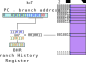
\includegraphics[width=\textwidth]{prediction_GShare-en.pdf}
\end{column}
\end{columns}
\end{frame}


\begin{frame}
\frametitle{Tournament predictors}

The basis of a tournament predictor is a competition between two other, simpler predictors. To choose which predictor is better, and therefore which predictor will be output, a 1-bit or 2-bit predictor can be used.

\bigskip
How the 1-bit tournament predictor works
\begin{itemize}
\item Calculate the prediction with predictors P1 and P2.
\item If the predictions match, this prediction is the result.
\item If the predictions do not match:
\begin{itemize}
\item The resulting prediction is whichever predictor has been successful in the past. This information is stored in a 1-bit state machine.
\item Select predictor P1 or P2 for the next prediction, depending on the fact.
\end{itemize}
\end{itemize}
\end{frame}

\begin{frame}
\frametitle{Tournament predictors}

\begin{center}
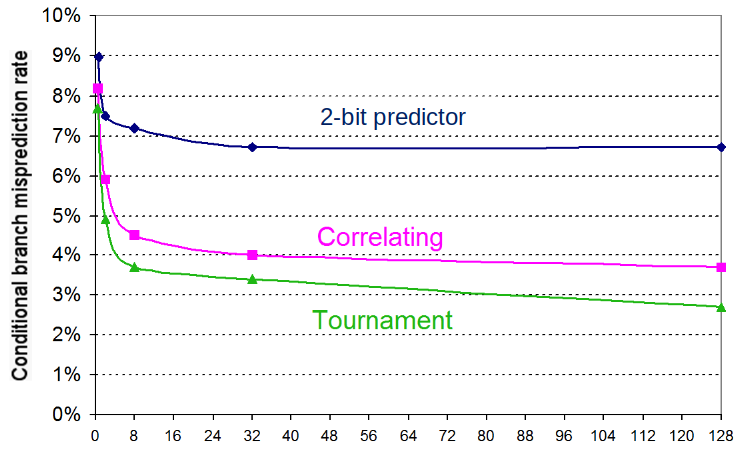
\includegraphics[width=0.75\textwidth]{fig/tournament.png}\\
\small Size of predictors in KiB
\end{center}
\end{frame}

\begin{frame}
\frametitle{Recap - quiz}

Which predictor can best predict the following fact of jumps if it starts in Taken or Weakly Taken state:

\begin{tabular}{|c|c|c|c|c|c|c|c|c|}\hline
T & T & T & NT & NT & NT& T & T & T \\ \hline
\end{tabular}

\bigskip
\begin{itemize}
 \item[A] 1-bit Smith predictor
 \item[B] 2-bit Smith predictor
 \item[C] 2-bit Smith predictor with hysteresis
 \item[D] all make the same number of errors
\end{itemize}
\end{frame}


\begin{frame}
\frametitle{Perceptron}

\begin{center}
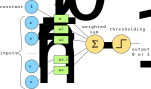
\includegraphics[width=0.6\textwidth]{neuron-en.pdf}
\end{center}

The formula $\xi = \sum_{i=0}^{n} x_i \cdot w_i$ is used to calculate the value. The final evaluation is by means of a transfer function, in our case a jump function, which has the form:
$f(\xi) = \begin{cases}1& \text{for }\xi \ge 0\\0& \text{for }\xi <0\end{cases}$
\end{frame}


\begin{frame}
\frametitle{AMD Zen2 predictor}

\begin{center}
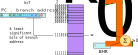
\includegraphics[width=0.7\textwidth]{prediction_amd-en.pdf}
\end{center}

According to the jump address, one perceptron is selected from the table.

The perceptron is defined by the weights $w_i$.

The prediction result is the sign of the weighted sum $\xi = \sum_{i=0}^{n} x_i \cdot w_i$, where $x_i$ are bits from the BHR jump history register.

Advantage -- better results than gshare, can be used for long BHR history registers, disadvantage -- complex calculation, cannot get the result in one CPU clock.
\end{frame}

\begin{frame}
\frametitle{AMD Zen2 -- Jump prediction}

\begin{itemize}
\item Calculating the perceptron output is relatively slow, normal perceptrons use real floating point numbers. It is possible to speed up with 16-bit real numbers, or by using a fixed decimal point.
\item The actual implementation of jump predictors has three levels
\begin{itemize}
\item level 1 -- 16 very fast predictors, deciding in the same clock cycle which other instructions to fetch
\item level 2 -- 512 predictors, which will refine the prediction in the next clock cycle, either discarding the loaded instructions or confirming them
\item level 3 -- 7168 predictors, in 4 hourly cycles refine the prediction. Again, the existing fetched instructions are either kept or discarded.
\end{itemize}
\item The average time delay for a bad final prediction is approximately 18 clock cycles.
\item At 4GHz and if every tenth instruction is a jump, a 1\% misprediction results in a performance degradation of almost 2\%.
\end{itemize}
\end{frame}


\begin{frame}
\frametitle{AMD Zen2 predictor}

\begin{center}
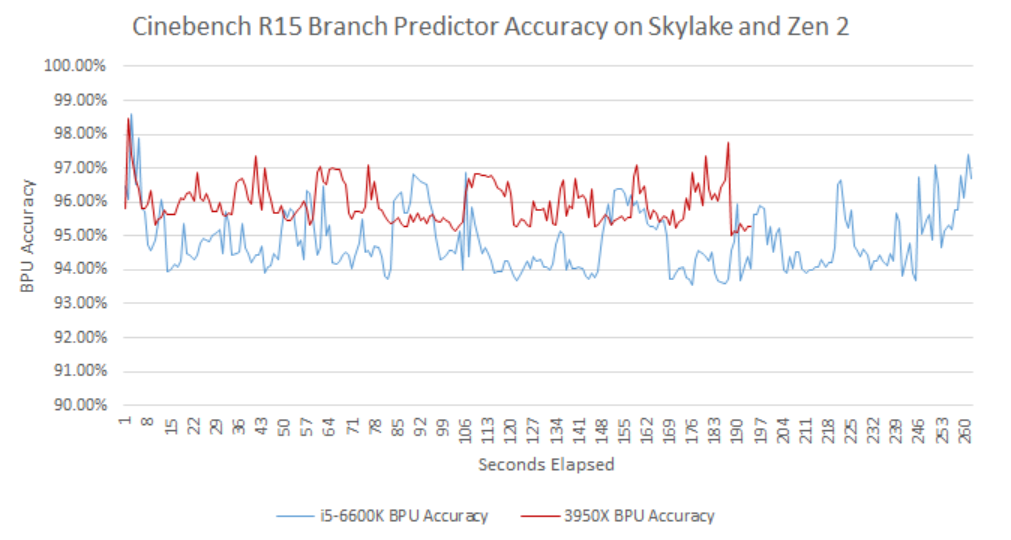
\includegraphics[width=0.8\textwidth]{fig/amd_cinebench.png}
\end{center}

Source: Analyzing Zen 2's Cinebench R15 Lead
By clamchowder from \url{https://chipsandcheese.com}
\end{frame}

\section{Target Prediction}

\begin{frame}
\frametitle{Jump target prediction}

Jumps have different jump target address formats in both RISC-V and other processors:
\begin{itemize}
\item jump to a fixed address -- the jump target is the address directly specified in the jump instruction (not in RISC-V because it has a fixed instruction length and a 32-bit address does not fit in the instruction code)
\item jump relative to the address of the jump instruction -- the jump target is calculated as the sum of the PC at the time the jump instruction is fetched and the specific value specified in the instruction.
\item jump to the position specified in the register or in memory -- RISC-V has the \texttt{jalr} instruction, i.e. jump to the address specified in the register, x86 contains the \texttt{ret} instruction -- return from the subroutine according to the address specified in memory on the stack and the \texttt{jump indirect} instruction, where the address points to the memory where the jump target address is specified (this instruction can be used when jumping according to a table, e.g. This can be used when compiling a \texttt{switch} construct, or when calling dynamic library functions).
\end{itemize}
\end{frame}

\begin{frame}
\frametitle{Jump target prediction}

\begin{itemize}
\item The jump target needs to be determined at the instruction fetch stage.
\item It is possible to have special dedicated adders for jump target addresses, but even there the summation takes some time.
\item Therefore it is important to estimate the jump target:
\begin{itemize}
\item BTB (Branch Target Buffer) is either a fully associative memory or a partially
associative with a given degree of associativity.
\item Lines are pairs:
\begin{itemize}
\item key -- BIA (Branch Instruction Address) -- i.e. the PC value at the time of the jump
\item BTA (Branch Target Address) -- the target address of the jump
\end{itemize}
\end{itemize}
\item If the PC matches the value of the BIA in the BTB and the predictor simultaneously predicts a jump, the PC is speculatively changed to the value of the corresponding BTA
\end{itemize}
\end{frame}

\begin{frame}
\frametitle{Function return prediction}

The most common jump by memory address is a return from function:
\begin{itemize}
\item For fast prediction of the return address of a function, modern CPUs contain a -- Return Address Stack (RAS)
\begin{itemize}
\item This is a fast stack memory -- remembering a limited number (up to 32) of return addresses
\item The value is stored in the RAS when the function is called, then when the ret instruction is fetched, the top of the RAS serves as a predictor of the jump target
\end{itemize}
\item Works reliably for function nesting levels depending on RAS size
\end{itemize}
\end{frame}

\section{Removing jumps from program}

\begin{frame}[fragile]
\frametitle{Example of how to remove a jump in a program}

You can find many tricks on the Internet to remove condition and therefore conditional jumps in your programs.

Here we will demonstrate removing the if from the calculation of the absolute value of an integer:

\begin{columns}[T]
\begin{column}{0.01\textwidth}
\phantom{x}
\end{column}
\begin{column}{0.25\textwidth}
program in C
\begin{minted}[fontsize=\small]{c}
if (x<0) {
  x = -x;
}
\end{minted}
\end{column}

\begin{column}{0.28\textwidth}
program in RISC-V
\begin{minted}[fontsize=\small]{gas}
 slt t0, s0, x0
 beq t0, x0, skip
 sub s0, x0, s0
skip:
\end{minted}
\end{column}
\begin{column}{0.45\textwidth}
\phantom{x}comment\
\small
compares whether x<0
will jump or not according to the result.
calculate -x
\end{column}
\end{columns}
\bigskip

To remove the conditional jump, which would be very hard to estimate, the following construction can be used, using the highest sign bit:
\begin{columns}[T]
\begin{column}{0.01\textwidth}
\phantom{x}
\end{column}
\begin{column}{0.25\textwidth}
program in C
\begin{minted}[fontsize=\small]{c}
int tmp = x>>31;
x^= tmp;
x -= tmp;
\end{minted}
\end{column}

\begin{column}{0.28\textwidth}
program in RISC-V
\begin{minted}[fontsize=\small]{gas}
srai t0, s0, 31
xor  s0, s0, t0
sub  s0, s0, t0
\end{minted}
\end{column}
\begin{column}{0.45\textwidth}
\phantom{x}comment\\
\small
tmp will be either 0 or 0xFFFFFFFFFF\\
does nothing, or bitwise inversion
for tmp==0 it does nothing, otherwise it subtracts -1, so it adds 1
\end{column}
\end{columns}
\end{frame}

\begin{frame}[fragile]
\frametitle{Example of how to remove a jump in a program}

If the value of b is 0 or 1, then the following C program can be executed:

\begin{minted}[fontsize=\small]{c}
a = ( (b!=0) ? c : d);
\end{minted}

change to program:

\begin{minted}[fontsize=\small]{c}
static const int lookup_table[] = {d,c};
a = lookup_table[b];
\end{minted}

\bigskip
Multiple jumps can also be removed at once, as long as again b1, b2, b3 only take values 0 or 1:

\begin{minted}[fontsize=\small]{c}
a = ( b1 ? c : ( b2 ? d : (b3 ? e : f)));
\end{minted}

can be changed to a program:

\begin{minted}[fontsize=\small]{c}
static const int lookup_table[] = { f, e, d, d, c, c, c, c };
a = lookup_table[b1 * 4 + b2 * 2 + b3];
\end{minted}
\end{frame}

\begin{frame}[fragile]
\frametitle{Example of how to remove a jump in a program}

Similarly, converting a number from 0 to 15 to a hex character can either
\begin{minted}[fontsize=\small]{c}
if (a<10) {
  ch = '0'+a;
} else {
  ch = 'A'+(a-10);
}
\end{minted}

can be changed to a program:

\begin{minted}[fontsize=\small]{c}
static const int hex_c[] = {'0','1','2','3','4','5','6','7',
                            '8','9','A','B','C','D','E','F'};
ch = hex_c[a];
\end{minted}
\end{frame}

\end{document}

